\documentclass{../../slides-style}

\slidetitleext[Computation Expressions, Workflows]{Вычислительные выражения в F\#}{20.03.2025}{Вычислительные выражения}

\begin{document}

    \begin{frame}[plain]
        \titlepage
    \end{frame}

    \section{Введение}

    \begin{frame}
        \frametitle{Что это и зачем нужно}
        \begin{itemize}
            \item Механизм управления процессом вычислений
            \begin{itemize}
                \item Обобщённые функции
            \end{itemize}
            \item В функциональных языках --- единственный способ определить порядок вычислений
            \item Зачастую --- нетривиальным образом (Async)
            \item Способ не писать кучу вспомогательного кода (сродни аспектно-ориентированному программированию)
            \item В теории ФП они называются монадами
            \item На самом деле, синтаксический сахар
        \end{itemize}
    \end{frame}

    \begin{frame}
        \frametitle{Пример}
        \framesubtitle{Классический пример с делением на 0}
        Сопротивление сети из параллельных резисторов:
        $$1/R = 1/R_1 + 1/R_2 + 1/R_3$$
        $R_1$, $R_2$ и $R_3$ могут быть 0. Что делать?
        \begin{itemize}
            \item Бросать исключение --- плохо
            \item Использовать option --- много работы, но попробуем
        \end{itemize}
    \end{frame}

    \begin{frame}[fragile]
        \frametitle{Реализация вручную}
        \framesubtitle{divide}
        \begin{minted}{fsharp}
let divide x y =
    match y with
    | 0.0 -> None
    | _ -> Some (x / y)
        \end{minted}
    \end{frame}

    \begin{frame}[fragile]
        \frametitle{Реализация вручную}
        \framesubtitle{Само вычисление}
        \begin{minted}{fsharp}
let resistance r1 r2 r3 =
    let r1' = divide 1.0 r1
    match r1' with
    | None -> None
    | Some x -> let r2' = divide 1.0 r2
        match r2' with
        | None -> None
        | Some y -> let r3' = divide 1.0 r3
            match r3' with
            | None -> None
            | Some z -> let r = divide 1.0 (x + y + z)
                        r
        \end{minted}
    \end{frame}

    \begin{frame}[fragile]{То же самое, через Workflow Builder}
        \begin{minted}{fsharp}
let resistance r1 r2 r3 = 
    maybe {
        let! r1' = divide 1.0 r1
        let! r2' = divide 1.0 r2
        let! r3' = divide 1.0 r3
        let! r = divide 1.0 (r1' + r2' + r3')
        return r
    }
        \end{minted}
    \end{frame}

    \begin{frame}[fragile]{seq --- это тоже Computation Expression}
        \begin{minted}{fsharp}
let daysOfTheYear =
    seq {
        let months =
            ["Jan"; "Feb"; "Mar"; "Apr"; "May"; "Jun";
             "Jul"; "Aug"; "Sep"; "Oct"; "Nov"; "Dec"]
        let daysInMonth month =
            match month with
            | "Feb" -> 28
            | "Apr" | "Jun" | "Sep" | "Nov" -> 30
            | _ -> 31
        for month in months do
            for day = 1 to daysInMonth month do
                yield (month, day)
    }
        \end{minted}
    \end{frame}

    \begin{frame}[fragile]
        \frametitle{Ещё один пример}
        \begin{minted}{fsharp}
let debug x = printfn "value is %A" x

let withDebug = 
    let a = 1
    debug a
    let b = 2
    debug b
    let c = a + b
    debug c
    c
        \end{minted}
    \end{frame}

    \begin{frame}[fragile]
        \frametitle{То же самое с Workflow}
        \begin{minted}{fsharp}
let withDebug = debugFlow {
        let! a = 1
        let! b = 2
        let! c = a + b
        return c
    }
        \end{minted}
    \end{frame}

    \section{Bind}

    \begin{frame}[fragile]{Как это сделать}
        \framesubtitle{let, \enquote{многословный} синтаксис}
        \begin{minted}{fsharp}
let x = something
        \end{minted}
        равносильно
        \begin{minted}{fsharp}
let x = something in [ выражение c x ]
        \end{minted}
        например,
        \begin{minted}{fsharp}
let x = 1 in
  let y = 2 in
    let z = x + y in
       z
        \end{minted}
    \end{frame}

    \begin{frame}[fragile]
        \frametitle{let и лямбды}
        \begin{minted}{fsharp}
fun x -> [ выражение c x ]
        \end{minted}
        или
        \begin{minted}{fsharp}
something |> (fun x -> [ выражение c x ])
        \end{minted}
        и обращаем внимание, что:
        \begin{minted}{fsharp}
let x = someExpression in [ выражение c x ]
someExpression |> (fun x -> [ выражение c x ])
        \end{minted}
    \end{frame}

    \begin{frame}[fragile]
        \frametitle{let и CPS}
        \begin{minted}{fsharp}
let x = 1 in
  let y = 2 in
    let z = x + y in
       z
        \end{minted}
        \begin{minted}{fsharp}
1 |> (fun x ->
  2 |> (fun y -> 
     x + y |> (fun z -> 
       z)))
        \end{minted}
    \end{frame}

    \begin{frame}[fragile]
        \frametitle{Можно обобщить до выполнения произвольного действия при вызове}
        \begin{minted}{fsharp}
let pipeInto expr f =
  expr |> f
        \end{minted}
        \begin{minted}{fsharp}
pipeInto (1, fun x ->
  pipeInto (2, fun y -> 
    pipeInto (x + y, fun z -> 
       z)))
        \end{minted}
    \end{frame}

    \begin{frame}[fragile]
        \frametitle{Зачем}
        \begin{minted}{fsharp}
let pipeInto (expr, f) =
   printfn "expression is %A" expr 
   expr |> f 
        \end{minted}
        \begin{minted}{fsharp}
pipeInto (1, fun x ->
  pipeInto (2, fun y -> 
    pipeInto (x + y, fun z -> 
       z)))
        \end{minted}
    \end{frame}

    \begin{frame}[fragile]
        \frametitle{То же самое с Workflow}
        \begin{minted}{fsharp}
type DebugBuilder() =
    member this.Bind(x, f) = 
        debug x 
        f x
    member this.Return(x) = x

let debugFlow = DebugBuilder ()

let withDebug = debugFlow {
        let! a = 1
        let! b = 2
        let! c = a + b
        return c
    }
        \end{minted}
    \end{frame}

    \begin{frame}[fragile]
        \frametitle{Более сложный пример, с делением}
        \framesubtitle{pipeInto, которая потом будет Bind}
        \begin{minted}{fsharp}
let pipeInto (expr, f) =
   match expr with
   | None -> 
       None
   | Some x -> 
       x |> f
        \end{minted}
    \end{frame}

    \begin{frame}[fragile]
        \frametitle{Более сложный пример, с делением}
        \framesubtitle{Сам процесс}
        \begin{minted}{fsharp}
let resistance r1 r2 r3 = 
    let a = divide 1.0 r1
    pipeInto (a, fun a' ->
        let b = divide 1.0 r2
        pipeInto (b, fun b' ->
            let c = divide 1.0 r3
            pipeInto (c, fun c' ->
                let r = divide 1.0 (a + b + c)
                pipeInto (r, fun r' ->
                    Some r
                ))))
        \end{minted}
    \end{frame}

    \begin{frame}[fragile]
        \frametitle{Уберём временные let-ы}
        \begin{minted}{fsharp}
let resistance r1 r2 r3 = 
    pipeInto (divide 1.0 r1, fun a ->
        pipeInto (divide 1.0 r2, fun b ->
            pipeInto (divide 1.0 r3, fun c ->
                pipeInto (divide 1.0 (a + b + c), fun r ->
                    Some r
                )))
        \end{minted}
    \end{frame}

    \begin{frame}[fragile]
        \frametitle{И отформатируем}
        \begin{minted}{fsharp}
let resistance r1 r2 r3 = 
    pipeInto (divide 1.0 r1, fun a ->
    pipeInto (divide 1.0 r2, fun b ->
    pipeInto (divide 1.0 r3, fun c ->
    pipeInto (divide 1.0 (a + b + c) , fun r ->
    Some r
    ))))
        \end{minted}
    \end{frame}

    \begin{frame}[fragile]
        \frametitle{Сравним с оригиналом}
        \begin{minted}{fsharp}
let resistance r1 r2 r3 = 
    maybe {
        let! r1' = divide 1.0 r1
        let! r2' = divide 1.0 r2
        let! r3' = divide 1.0 r3
        let! r = divide 1.0 (r1' + r2' + r3')
        return r
    }
        \end{minted}
    \end{frame}
    
    \section{Как работают CE}

    \begin{frame}{WorkflowBuilder}
        \begin{itemize}
            \item Bind создаёт цепочку continuation passing style-функций, возможно, с побочными эффектами
            \item Есть тип-обёртка (или монадический тип), в котором хранится состояние вычисления
            \begin{itemize}
                \item Или, более функционально, которое представляет \emph{действие} при вычислении
            \end{itemize}
            \item let! вызывает Bind, return --- Return, Bind принимает обёрнутое значение и функцию-continuation, return по необёрнутому значению делает обёрнутое
            \begin{itemize}
                \item На самом деле, это просто композиция функций, но хитрая, потому что монадический тип
            \end{itemize} 
            \item WorkflowBuilder --- это просто класс, в котором должны лежать методы с нужными сигнатурами, сам workflow --- объект этого класса
            \begin{itemize}
                \item Обычно он один, но в теории ничто не мешает хранить в нём побочные эффекты
                \item Не путайте WorkflowBuilder с монадическим типом, это другое
            \end{itemize}
        \end{itemize}
    \end{frame}

    \begin{frame}{Railway-oriented programming}
        \framesubtitle{Монадический тип может управлять вычислением}
        \begin{center}
            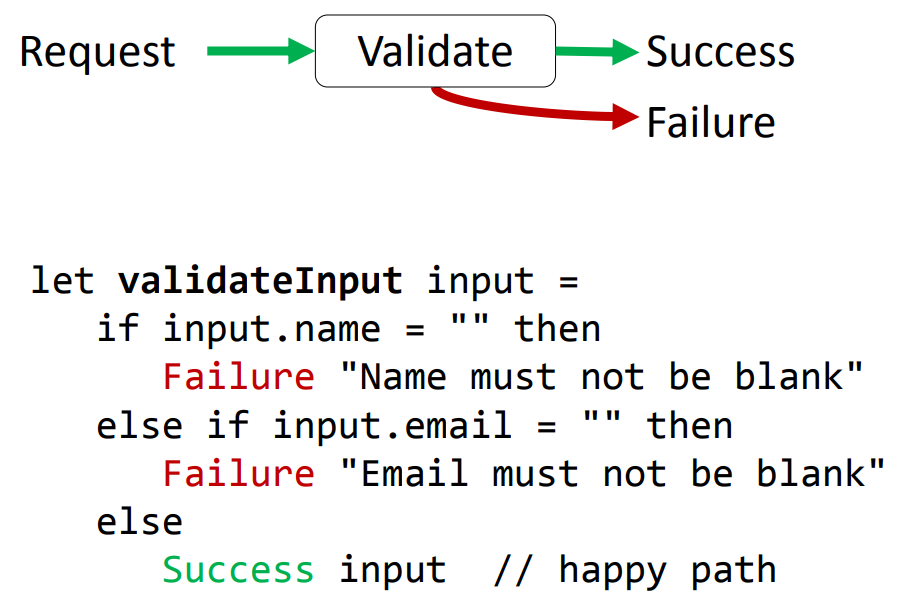
\includegraphics[width=0.6\textwidth]{validationExample.png}

            \vspace{0.5cm}

            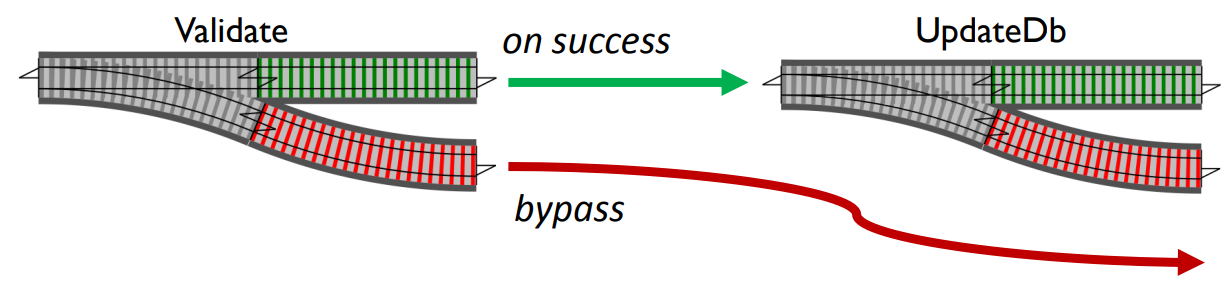
\includegraphics[width=0.7\textwidth]{railroads.png}
        \end{center}
    \end{frame}

    \begin{frame}{Что на самом деле делает Bind}
        \begin{center}
            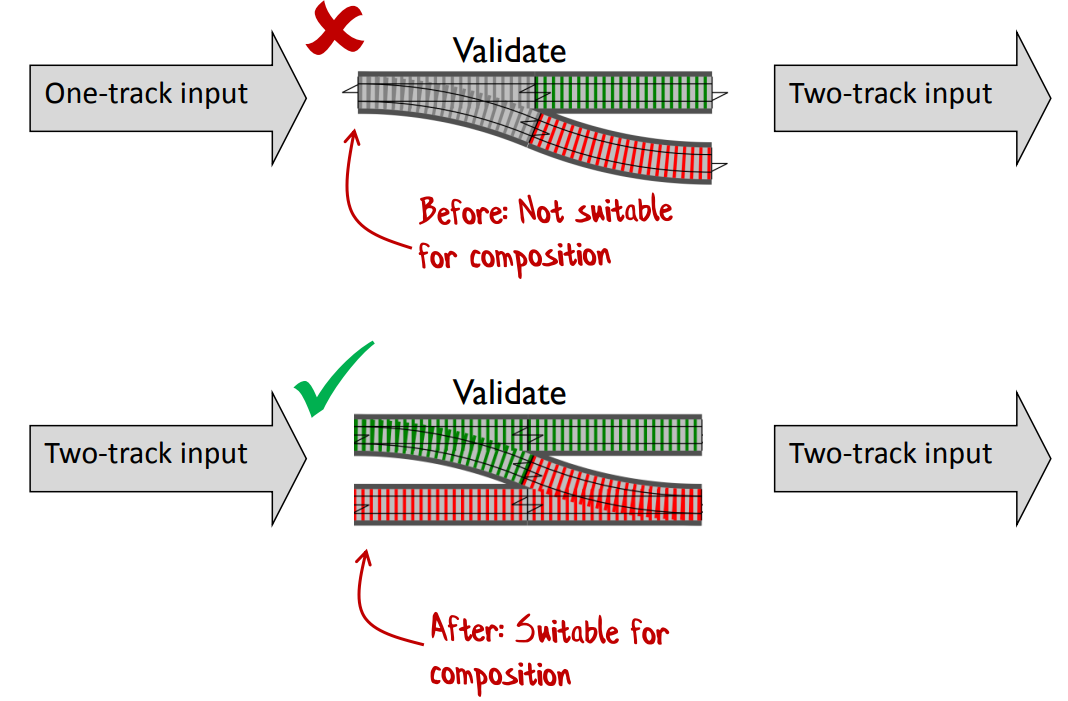
\includegraphics[width=0.7\textwidth]{bindRailroads.png}
        \end{center}

        \attribution{\url{https://github.com/swlaschin/RailwayOrientedProgramming/blob/master/Railway_Oriented_Programming_Slideshare.pdf}}
    \end{frame}

    \begin{frame}[fragile]
        \frametitle{Подробнее про Bind}
        \begin{itemize}
            \item Bind : M<'T> * ('T -> M<'U>) -> M<'U>
            \item Return : 'T -> M<'T>
        \end{itemize}
        \begin{minted}{fsharp}
let! x = 1 in x * 2
        \end{minted}
        \begin{minted}{fsharp}
builder.Bind(1, (fun x -> x * 2))
        \end{minted}
    \end{frame}

    \begin{frame}[fragile]
        \frametitle{Инфиксное определение Bind}
        \frametitle{Как в Haskell}
        \begin{minted}{fsharp}
let (>>=) m f = pipeInto(m, f)

let workflow = 
    1 >>= (+) 2 >>= (*) 42 >>= id
        \end{minted}
    \end{frame}

    \begin{frame}[fragile]
        \frametitle{Option.bind и maybe}
        \begin{minted}{fsharp}
module Option = 
    let bind f m =
       match m with
       | None -> 
           None
       | Some x -> 
           x |> f 

type MaybeBuilder() =
    member this.Bind(m, f) = Option.bind f m
    member this.Return(x) = Some x
        \end{minted}
    \end{frame}

    \section{Монадический тип}

    \begin{frame}[fragile]
        \frametitle{Содержимое типа-обёртки может иметь разный тип}
        \framesubtitle{Пример, серия запросов к БД}
        \begin{minted}{fsharp}
type DbResult<'a> = 
    | Success of 'a
    | Error of string

type CustomerId =  CustomerId of string
type OrderId =  OrderId of int
type ProductId =  ProductId of string
        \end{minted}
    \end{frame}

    \begin{frame}[fragile]
        \frametitle{Пример, запросы}
        \begin{minted}{fsharp}
let getCustomerId name =
    if (name = "") 
    then Error "getCustomerId failed"
    else Success (CustomerId "Cust42")

let getLastOrderForCustomer (CustomerId custId) =
    if (custId = "") 
    then Error "getLastOrderForCustomer failed"
    else Success (OrderId 123)

let getLastProductForOrder (OrderId orderId) =
    if (orderId  = 0) 
    then Error "getLastProductForOrder failed"
    else Success (ProductId "Product456")
        \end{minted}
    \end{frame}

    \begin{frame}[fragile]
        \frametitle{Общение с БД вручную}
        \begin{minted}{fsharp}
let product = 
    let r1 = getCustomerId "Alice"
    match r1 with 
    | Error e -> Error e
    | Success custId ->
        let r2 = getLastOrderForCustomer custId 
        match r2 with 
        | Error e -> Error e
        | Success orderId ->
            let r3 = getLastProductForOrder orderId 
            match r3 with 
            | Error e -> Error e
            | Success productId ->
                printfn "Product is %A" productId
                r3
        \end{minted}
    \end{frame}

    \begin{frame}[fragile]
        \frametitle{Builder}
        \begin{minted}{fsharp}
type DbResultBuilder() =

    member this.Bind(m, f) = 
        match m with
        | Error e -> Error e
        | Success a -> 
            printfn "Successful: %A" a
            f a

    member this.Return(x) = 
        Success x

let dbresult = new DbResultBuilder()
        \end{minted}
    \end{frame}

    \begin{frame}[fragile]
        \frametitle{Workflow}
        \begin{minted}{fsharp}
let product = 
    dbresult {
        let! custId = getCustomerId "Alice"
        let! orderId = getLastOrderForCustomer custId
        let! productId = getLastProductForOrder orderId 
        printfn "Product is %A" productId
        return productId
    }
printfn "%A" product
        \end{minted}
    \end{frame}

    \section{Композиция}

    \begin{frame}[fragile]
        \frametitle{Композиция Workflow-ов}
        \begin{minted}{fsharp}
let subworkflow1 = myworkflow { return 42 }
let subworkflow2 = myworkflow { return 43 }

let aWrappedValue = 
    myworkflow {
        let! unwrappedValue1 = subworkflow1
        let! unwrappedValue2 = subworkflow2
        return unwrappedValue1 + unwrappedValue2
    }
        \end{minted}
    \end{frame}

    \begin{frame}[fragile]
        \frametitle{Вложенные Workflow-ы}
        \begin{minted}{fsharp}
let aWrappedValue = 
    myworkflow {
        let! unwrappedValue1 = myworkflow {
            let! x = myworkflow { return 1 }
            return x
        }
        let! unwrappedValue2 = myworkflow {
            let! y = myworkflow { return 2 }
            return y
        }
        return unwrappedValue1 + unwrappedValue2
    }
        \end{minted}
    \end{frame}

    \begin{frame}[fragile]
        \frametitle{ReturnFrom}
        \begin{minted}{fsharp}
type MaybeBuilder() =
    member this.Bind(m, f) = Option.bind f m
    member this.Return(x) = 
        printfn "Wrapping a raw value into an option"
        Some x
    member this.ReturnFrom(m) = 
        printfn "Returning an option directly"
        m

let maybe = new MaybeBuilder()
        \end{minted}
    \end{frame}

    \begin{frame}[fragile]
        \frametitle{Пример}
        \begin{minted}{fsharp}
maybe { return 1  }

maybe { return! (Some 2)  }
        \end{minted}
    \end{frame}

    \begin{frame}[fragile]
        \frametitle{Зачем это}
        \begin{minted}{fsharp}
maybe {
    let! x = divide 24 3
    let! y = divide x 2
    return y 
}

maybe {
    let! x = divide 24 3
    return! divide x 2  
}
        \end{minted}
    \end{frame}

    \section{Законы монад}

    \begin{frame}[fragile]
        \frametitle{Первый и второй законы монад}
        \begin{itemize}
            \item Bind и Return должны быть взаимно обратны
        \end{itemize}
        \begin{footnotesize}
            \begin{minted}{fsharp}
myworkflow {
    let originalUnwrapped = something
    let wrapped = myworkflow { return originalUnwrapped }
    let! newUnwrapped = wrapped
    assertEqual newUnwrapped originalUnwrapped 
}
myworkflow {
    let originalWrapped = something
    let newWrapped = myworkflow { 
        let! unwrapped = originalWrapped
        return unwrapped
    }
    assertEqual newWrapped originalWrapped
}
            \end{minted}
        \end{footnotesize}
    \end{frame}

    \begin{frame}[fragile]
        \frametitle{Или то же самое на Haskell}
        \begin{minted}{haskell}
return x >>= f == f x
mv >>= return == mv
        \end{minted}
        \vspace{5mm}
        Или через монадную композицию (\mintinline{haskell}|f >=> g = \x -> (f x >>= g)|):
        \begin{minted}{haskell}
return >=> f == f
f >=> return == f
        \end{minted}
        \vspace{5mm}
        В Haskell монады синтаксически приятнее
    \end{frame}

    \begin{frame}[fragile]
        \frametitle{Третий закон монад}
        \begin{itemize}
            \item Ассоциативность композиции
        \end{itemize}
        \begin{minted}{fsharp}
let result1 = myworkflow { 
    let! x = originalWrapped
    let! y = f x 
    return! g y  
}
let result2 = myworkflow { 
    let! y = myworkflow { 
        let! x = originalWrapped
        return! f x
    }
    return! g y
}
assertEqual result1 result2
        \end{minted}
    \end{frame}

    \begin{frame}[fragile]
        \frametitle{Или на Haskell}
        \begin{minted}{haskell}
(mv >>= f) >>= g == mv >>= (\x -> (f x >>= g))
        \end{minted}
        \vspace{5mm}
        Или через композицию:
        \begin{minted}{haskell}
(f >=> g) >=> h == f >=> (g >=> h)
        \end{minted}
        \vspace{5mm}

        Три закона монад обеспечивают адекватность их композиции.
    \end{frame}

    \section{Методы WorkflowBuilder}

    \begin{frame}
        \frametitle{Какие ещё методы есть у WorkflowBuilder}
        \begin{footnotesize}
            \begin{tabu} {| X[0.5 l p] | X[1 l p] | X[1 l p] |}
                \tabucline-
                Имя                      & Тип                                                 & Описание                    \\
                \tabucline-
                \everyrow{\tabucline-}
                Delay                    & (unit -> M<'T>) -> M<'T>                            & Превращает в функцию        \\
                Run                      & M<'T> -> M<'T>                                      & Исполняет вычисление        \\
                Combine                  & M<'T> * M<'T> -> M<'T>                              & Последовательное исполнение \\
                For                      & seq<'T> * ('T -> M<'U>) -> M<'U>                    & Цикл for                    \\
                TryWith                  & M<'T> * (exn -> M<'T>) -> M<'T>                     & Блок try with               \\
                TryFinally               & M<'T> * (unit -> unit) -> M<'T>                     & Блок finally                \\
                Using                    & 'T * ('T -> M<'U>) -> M<'U> when 'U :> IDisposable  & use                         \\
                While                    & (unit -> bool) * M<'T> -> M<'T>                     & Цикл while                  \\
                Yield                    & 'T -> M<'T>                                         & yield или ->                \\
                YieldFrom                & M<'T> -> M<'T>                                      & yield! или ->>              \\
                Zero                     & unit -> M<'T>                                       & Обёрнутое ()                \\
            \end{tabu}
        \end{footnotesize}
    \end{frame}

    \begin{frame}{Подробнее про Run и Delay}
        Результат вычисления выражения:

        \vspace{1cm}

        \begin{center}
            \mintinline{text}|builder.Run(builder.Delay(fun () -> {{ cexpr }}))|
        \end{center}
    \end{frame}

    \section{Пример DSL на Workflow}

    \begin{frame}[fragile]{Пример, DSL для создвния презентаций}
        \begin{minted}{fsharp}
// Доменная модель
type Slide = { Header: string }

type Deck = { Title: string; Slides: Slide list }

// WorkflowBuilder
type SlideBuilder() =
    member inline _.Yield(()) = ()

    // Можно определять свои операции!
    // ... но нужен yield
    [<CustomOperation("header")>]
    member inline _.Header((), header: string) : Slide = 
        { Header = header }

let slide = SlideBuilder()
        \end{minted}
    \end{frame}

    \begin{frame}[fragile]
        \frametitle{Как использовать}
        \begin{minted}{fsharp}
slide {
    header "Hello world!"
}
        \end{minted}
    \end{frame}

    \begin{frame}[fragile]{Сделаем генерацию Deck}
        \begin{minted}{fsharp}
[<RequireQualifiedAccess>]
type DeckProperty =
    | Title of string

type DeckBuilder() =
    member inline _.Yield(()) = ()
    member inline _.Run(DeckProperty.Title title) = { Title = title; Slides = [] }

    [<CustomOperation("title")>]
    member inline _.Title((), title: string) = DeckProperty.Title title

let deck = DeckBuilder()
        \end{minted}
    \end{frame}

    \begin{frame}[fragile]
        \frametitle{Сделаем генерацию слайдов (пока одного)}
        \begin{minted}{fsharp}
[<RequireQualifiedAccess>]
type DeckProperty = Title of string | Slide of Slide

type DeckBuilder() =
    member inline _.Yield(()) = ()
    member inline _.Yield(slide: Slide) = DeckProperty.Slide slide

    member inline _.Run(prop) =
        match prop with
        | DeckProperty.Title title -> { Title = title; Slides = [] }
        | DeckProperty.Slide slide -> { Title = ""; Slides = [ slide ] }

    [<CustomOperation("title")>]
    member inline _.Title((), title: string) = DeckProperty.Title title
        \end{minted}
    \end{frame}

    \begin{frame}[fragile]
        \frametitle{Как использовать}
        \begin{minted}{fsharp}
deck {
    yield slide {
        header "Hello world!"
    }
}
        \end{minted}
    \end{frame}

    \begin{frame}[fragile]
        \frametitle{Сделаем цепочку слайдов}
        \begin{footnotesize}
            \begin{minted}{fsharp}
type DeckBuilder() =
    (* ... *)

    member inline _.Delay(f: unit -> DeckProperty list) = f()
    member inline _.Delay(f: unit -> DeckProperty) = [f ()]

    member inline _.Combine(newProp: DeckProperty, 
            previousProps: DeckProperty list) =
        newProp :: previousProps

    member inline x.Run(props: DeckProperty list) =
        props
        |> List.fold
            (fun deck prop ->
                match prop with
                | DeckProperty.Title title -> { deck with Title = title }
                | DeckProperty.Slide slide -> { deck with Slides = slide :: deck.Slides })
            { Title = ""; Slides = [] }

    member inline x.Run(prop: DeckProperty) = x.Run([prop])
            \end{minted}
        \end{footnotesize}
    \end{frame}

    \begin{frame}[fragile]{Теперь можно так}
        \begin{minted}{fsharp}
deck {
    title "Testing Deck with title"

    slide {
        header "This works"
    }

    slide {
        header "...and also this!"
    }

    slide {
        header "Much wow!"
    }
}
        \end{minted}
        Но надо ещё For
    \end{frame}

    \begin{frame}[fragile]{Итого}
        \begin{ssmall}
            \begin{minted}{fsharp}
[<RequireQualifiedAccess>]
type DeckProperty =
    | Title of string
    | Slide of Slide

type DeckBuilder() =
    member inline _.Yield(()) = ()
    member inline _.Yield(slide: Slide) = DeckProperty.Slide slide

    member inline _.Delay(f: unit -> DeckProperty list) = f ()
    member inline _.Delay(f: unit -> DeckProperty) = [ f () ]

    member inline _.Combine(newProp: DeckProperty, previousProps: DeckProperty list) = newProp :: previousProps

    member inline x.For(prop: DeckProperty, f: unit -> DeckProperty list) = x.Combine(prop, f ())
    member inline x.For(prop: DeckProperty, f: unit -> DeckProperty) = [prop; f()]

    member inline x.Run(props: DeckProperty list) =
        props
        |> List.fold
            (fun deck prop ->
                match prop with
                | DeckProperty.Title title -> { deck with Title = title }
                | DeckProperty.Slide slide -> { deck with Slides = deck.Slides @ [ slide ] })
            { Title = ""; Slides = [] }

    member inline x.Run(prop: DeckProperty) = x.Run([ prop ])

    [<CustomOperation("title")>]
    member inline _.Title((), title: string) = DeckProperty.Title title
            \end{minted}
        \end{ssmall}
    \end{frame}

    \section{Моноиды и эндоморфизмы}

    \begin{frame}
        \frametitle{Моноиды}
        \framesubtitle{Немного алгебры}
        Множество с бинарной операцией
        \begin{itemize}
            \item Замкнутость относительно операции
            \item Ассоциативность
            \item Наличие нейтрального элемента
        \end{itemize}
        Например, [a] @ [b] = [a; b]
    \end{frame}

    \begin{frame}[fragile]
        \frametitle{Пример}
        \begin{minted}{fsharp}
type OrderLine = {Quantity : int; Total : float}

let orderLines = [
    {Quantity = 2; Total = 19.98};
    {Quantity = 1; Total = 1.99};
    {Quantity = 2; Total = 3.98}; ]
    
let addLine line1 line2 =
    {Quantity = line1.Quantity + line2.Quantity; 
     Total = line1.Total + line2.Total}
     
orderLines |> List.reduce addLine
        \end{minted}
    \end{frame}

    \begin{frame}
        \frametitle{Эндоморфизмы}
        Эндоморфизм --- функция, у которой тип входного значения совпадает с типом выходного
        
        \vspace{1cm}
        Множество функций + композиция --- моноид, если функции --- эндоморфизмы
    \end{frame}

    \begin{frame}[fragile]
        \frametitle{Пример}
        \begin{minted}{fsharp}
let plus1 x = x + 1
let times2 x = x * 2
let subtract42 x = x - 42

let functions = [
    plus1;
    times2;
    subtract42 ]

let newFunction = functions |> List.reduce (>>)

printfn "%d" <| newFunction 20
        \end{minted}
    \end{frame}

    \begin{frame}[fragile]
        \frametitle{Не только эндоморфизмы могут образовать моноид}
        \begin{minted}{fsharp}
type Predicate<'A> = 'A -> bool

let predAnd p1 p2 x = 
    if p1 x 
    then p2 x
    else false

let predicates = [isMoreThan10Chars; isMixedCase; 
                  isNotDictionaryWord]

let combinePredicates = predicates |> List.reduce predAnd
        \end{minted}
    \end{frame}

    \section{Полезные ссылки}

    \begin{frame}
        \frametitle{Полезные ссылки}
        \framesubtitle{Откуда взяты примеры}
        \begin{small}
            \begin{itemize}
                \item \url{https://fsharpforfunandprofit.com/series/computation-expressions.html} --- описание Workflow-ов в F\# без использования слова \enquote{монада}
                \item \url{https://fsharpforfunandprofit.com/fppatterns/} --- отличная презентация про ФП вообще, включая Railroad programming и монады
                \item \url{https://habr.com/ru/articles/127556/} --- перевод статьи с простым объяснением монад в Haskell
                \item \url{https://sleepyfran.github.io/blog/posts/fsharp/ce-in-fsharp/} --- пример с DSL на Workflow-ах
            \end{itemize}
        \end{small}
    \end{frame}

\end{document}
